\documentclass[10.5pt]{article}
\usepackage{drp_preamble}



\fancyhead{}
\fancyhead[L]{DRP: Your name}
\fancyhead[R]{\thepage}
\renewcommand{\headrulewidth}{0.4pt}
\renewcommand{\footrulewidth}{0pt}

\addbibresource{references.bib}

\graphicspath{ {Images/} } % Tell the main.tex which directory to look for figures/ images

\newtheorem{theorem}{Theorem} %[section]

% Begin document
\begin{document}
% First page different, no numbering (Title page)
\fancyfoot{}
\pagenumbering{gobble}
\pagestyle{plain}
\begin{titlepage}
    \begin{center}
        

        \begin{figure}[H]
            \centering
            \makebox[0.85\textwidth]{
\includegraphics[width=0.85\linewidth]{wvu_logo.pdf}}
        \end{figure}

        %\vfill
        \normalsize	    
        \textbf{Benjamin M. Statler College of} \\
        \textbf{Engineering and Mineral Resources} \\
        \textbf{Department of Chemical and Biomedical Engineering} \\
        \vspace{1.0cm}

        \huge
        \textbf{DISSERTATION} \\
        \textbf{RESEARCH} \\
        \textbf{PROPOSAL} \\
        \vspace{1.0cm}

        \normalsize	
        \uppercase{\textbf{Title of your Disseration here}}
            
        \vspace{1.0cm}

        \normalsize
        Research Advisor: Dr. Fernando V. Lima\\
        Ph.D. Student: Your name\\
        \vspace{1.5cm}
        \vfill
        Morgantown, Jan 1, 2024\\
        
        \vfill
        Keywords: add, keywords, related, to your work \\
        \vspace{0.5cm}
        \textbf{Copyright 2023 Your Name}
    \end{center}
\end{titlepage}


% Front matter: Project Summary, Intellectual Merit, Broader Impacts.
\pagenumbering{arabic}
\pagestyle{fancy}
\underline{\textbf{Project Summary:}} Here you will summarize the research in a short paragraph. This whole section should be roughly one-page long. 

\vspace{5mm} %5mm vertical space, delete this when working on your DRP.


\lipsum[1]

\vspace{5mm} %5mm vertical space, delete this when working on your DRP.

\underline{\textbf{Intellectual Merit:}} Describe the intellectual merit of your research with references. 

\vspace{5mm} %5mm vertical space, delete this when working on your DRP.


\lipsum[1]

\vspace{5mm} %5mm vertical space, delete this when working on your DRP.

\underline{\textbf{Broader Impacts:}} What are the broader impacts and main contributions? State them here clearly. 

\vspace{5mm} %5mm vertical space, delete this when working on your DRP.

\lipsum[1]

\vspace{5mm} %5mm vertical space, delete this when working on your DRP.


 
\pagebreak

\pagestyle{fancy}
\section{Overview and Objectives}\label{chapter: overview}

In this section, you should give an overview of your research topic with relevant citations, and clearly state your research aims.

\vspace{5mm} %5mm vertical space, delete this when working on your DRP.

\textbf{Specific aim \#1: Your first aim.} \lipsum[1-2]

\textbf{Specific aim \#2: Your second aim.} \lipsum[1-2]

\textbf{Specific aim \#3: Your third aim.} \lipsum[1-2]

\textbf{Specific aim \#4: Your fourth aim.} \lipsum[1-2]

 

\pagestyle{fancy}
\section{Expected Significance}\label{chapter: significance}
What is the expected significance of your research? This is the place to summarize this. See the example in the repository. 

\pagestyle{fancy}
\section{Literature Review}\label{chapter: review}
Here you should add the literature review related to your research field. See the example.

Some references can be cited \cite{alves2018,alves2022,alves2023}. You should add your licenses in the references.bib file. You should delete the references from there, and your own \cite{alves2022}.

\lipsum[1-5] 

\pagestyle{fancy}
\section{Background}\label{chapter: content1}

\subsection{Subsection}


Example of a subsection. Equation below for illustration purposes.


\begin{equation}
    M=\left\{\begin{array}{l}
        \dot{x}_{s}=f\left(x_{s}, u, d\right) \\
        y=g\left(x_{s}, u, d\right) \\
        h_{1}\left(\dot{x}_{s}, x_{s}, y, \dot{u}, u, d\right)=0 \\
        h_{2}\left(\dot{x}_{s}, x_{s}, y, \dot{u}, u, d\right) \geq 0
    \end{array}\right.
    \label{eq:eq1}
\end{equation}

Example of a table.


\begin{table}[H]
    \caption{Steady-state operability sets: definitions and mathematical formulations.}
    \label{tab:my-table1}
    \resizebox{\textwidth}{!}{%
    \begin{tabular}{|c|c|c|}
    \hline
    \textbf{Operability Set}                                                                     & \textbf{Description}                                                                                                                                                                                                         & \textbf{Mathematical Formulation}                                                                                                                                                                                    \\ \hline
    \textbf{\begin{tabular}[c]{@{}c@{}}Available \\ Input Set (AIS)\end{tabular}}                & \begin{tabular}[c]{@{}c@{}}Manipulated inputs ($ u \in \mathbb{R}^m$) \\ based on the design of the process that is limited \\ by the process constraints \cite{vinson00}.\end{tabular}                                              & $\mathrm{AIS}=\left\{u \mid u_{i}^{\min } \leq u_{i} \leq u_{i}^{\max } ; 1 \leq i \leq m\right\}$                                                                                                                   \\ \hline
    \textbf{\begin{tabular}[c]{@{}c@{}}Expected \\ Disturbance \\ Set (EDS)\end{tabular}}        & \begin{tabular}[c]{@{}c@{}}Disturbance variables ($d \in \mathbb{R}^q$) that \\ can represent process uncertainties and variabilities.\end{tabular}                                                                                   & $\mathrm{EDS}=\left\{d \mid d_{i}^{\min } \leq d_{i} \leq d_{i}^{\max } ; 1 \leq i \leq q\right\}$                                                                                                                   \\ \hline
    \textbf{\begin{tabular}[c]{@{}c@{}}Achievable \\ Output Set \\ (AOS)\end{tabular}}           & \begin{tabular}[c]{@{}c@{}}Range of the outputs ($y \in \mathbb{R}^n$) \\ that can be achieved using \\ the inputs inside the AIS and disturbances within the EDS.\end{tabular}                                                                                          & $\operatorname{AOS}(d)=\{y \mid y=M(u, d) ; u \in$ AIS, $d$ is fixed$\}$                                                                                                                                            \\ \hline
    \textbf{\begin{tabular}[c]{@{}c@{}}Desired \\ Output Set \\ (DOS)\end{tabular}}              & \begin{tabular}[c]{@{}c@{}}Production/target/efficiency \\ requirements for the outputs that do not \\ necessarily meet the ranges of the AOS.\end{tabular}                                                                  & DOS $=\left\{y \mid y_{i}^{\min } \leq y_{i} \leq y_{i}^{\max } ; 1 \leq i \leq n\right\}$                                                                                                                           \\ \hline
    \textbf{\begin{tabular}[c]{@{}c@{}}Desired \\ Input Set \\ (DIS)\end{tabular}}               & \begin{tabular}[c]{@{}c@{}}Set of inputs required to reach the entire DOS, \\ given a disturbance vector \textit{d}.\end{tabular}                                                                                           & $\operatorname{DIS}(d)=\left\{u \mid u=M^{-1}(y, d) ; y \in \mathrm{DOS}, d\right.$ is fixed$\}$                                                                                                                    \\ \hline
    \textbf{\begin{tabular}[c]{@{}c@{}}Feasible \\ Desired \\ Output Set \\ (DOS*)\end{tabular}} & \begin{tabular}[c]{@{}c@{}}Feasible set of desired outputs calculated via \\ relative error minimization \\ from the DOS using for example the \\ NLP-based approach \cite{carrasco2017}.\end{tabular}                  & $\mathrm{DOS}^{*}=\left\{y^{*} \mid y^{*}=M\left(u^{*}\right) ; u^{*} \in \mathrm{DIS}^{*}\right\}$                                                                                                                  \\ \hline
    \textbf{\begin{tabular}[c]{@{}c@{}}Feasible \\ Desired \\ Input Set \\ (DIS*)\end{tabular}}  & \begin{tabular}[c]{@{}c@{}}Optimal set of inputs that are required to obtain the \\ Feasible Desired Output Set (DOS*), \\ calculated for example via the NLP-based approach.\end{tabular}                               & \begin{tabular}[c]{@{}c@{}}$\mathrm{DIS}^{*}=\left\{u^{*} \mid u^{*}=\left(u_{1}^{*}, u_{2}^{*}, u_{3}^{*} \ldots u_{i}^{*}\right)\right\}$\\ $i \stackrel{\text { def }}{=}$ Discretized DOS grid size\end{tabular} \\ \hline
    \end{tabular}%
    }
\end{table}


\subsection{Another subsection!}

If you need several subsections, this might help you. Equation below as an example as well.


\begin{equation}
    \widehat{Y}_{l}(u)=\mathcal{F}(u)+z_{l}(u), \quad l=1, \ldots, p
    \label{eq:kr1}
\end{equation} 

\pagestyle{fancy}

\pagestyle{fancy}
\subsection{Control Structure Selection}\label{chapter: content2}
Add content related to your DRP here as well.

\vspace{5mm} %5mm vertical space, delete this when working on your DRP.

\lipsum[1-5] 

\pagestyle{fancy}
\section{Preliminary Results}\label{chapter: results}
Here you should summarize your findings, according to each aim.

\subsection{Aim \# 1:Your first aim}

\lipsum[1-3]



\subsubsection{Subsection of your first aim}


\lipsum[1-3]


\subsection{Aim \#2: Your second aim} \label{section:ad-based-op}

\lipsum[1-3]

	\subsubsection{Subsection of your second aim}

	\lipsum[1-3]

\subsection{Aim \#3: Your third aim} 

\lipsum[1-3]

\begin{enumerate}
	\item example of itemized list.
	\item example of itemized list.
\end{enumerate}



\subsubsection{Another subsection}

\lipsum[1-2]



\pagestyle{fancy}
\section{Research Plan}\label{chapter: plan}
Here you will detail your research plan that your presented previously, going into more details on how do you plan to achieve your goals.

\vspace{5mm} %5mm vertical space, delete this when working on your DRP.

\textbf{Specific aim \#1: Your first aim.} \lipsum[1-3]

\begin{enumerate}
    \item \underline{Substask related to your first aim}: \lipsum[1-3]
    \item \underline{Second substask related to your first aim}: \lipsum[1-3]

    \item \underline{Third substask related to your first aim:} \lipsum[1-3]
\end{enumerate}

\textbf{Specific aim \#2: Your second aim.} \lipsum[1-3]
\begin{enumerate}
    \item \underline{Substask related to your second aim:} \lipsum[1-3]
    \item \underline{Second substask related to your second aim::} \lipsum[1-3]
\end{enumerate}

\textbf{Specific aim \#3: Your third aim.} \lipsum[1-3]

\begin{enumerate}
    \item \underline{Substask related to your third aim (completed):} \lipsum[1-3]
    \item \underline{Second substask related to your third aim:} \lipsum[1-3]
\end{enumerate}


\textbf{Specific aim \#4: Your last aim.} \lipsum[1-3]

\begin{enumerate}
    \item \underline{Substask related to your last aim (completed):} \lipsum[1-3]
    \item \underline{Substask (completed):} \lipsum[1-3]
    \item \underline{Substask 2 (completed):} \lipsum[1-3]
    \item \underline{Substask 3 (completed):} \lipsum[1-3].
   
\end{enumerate}


\pagestyle{fancy}
\section{Timeline}\label{chapter: timeline}
\begin{figure}[H]
    \centering
    \makebox[0.95\textwidth]{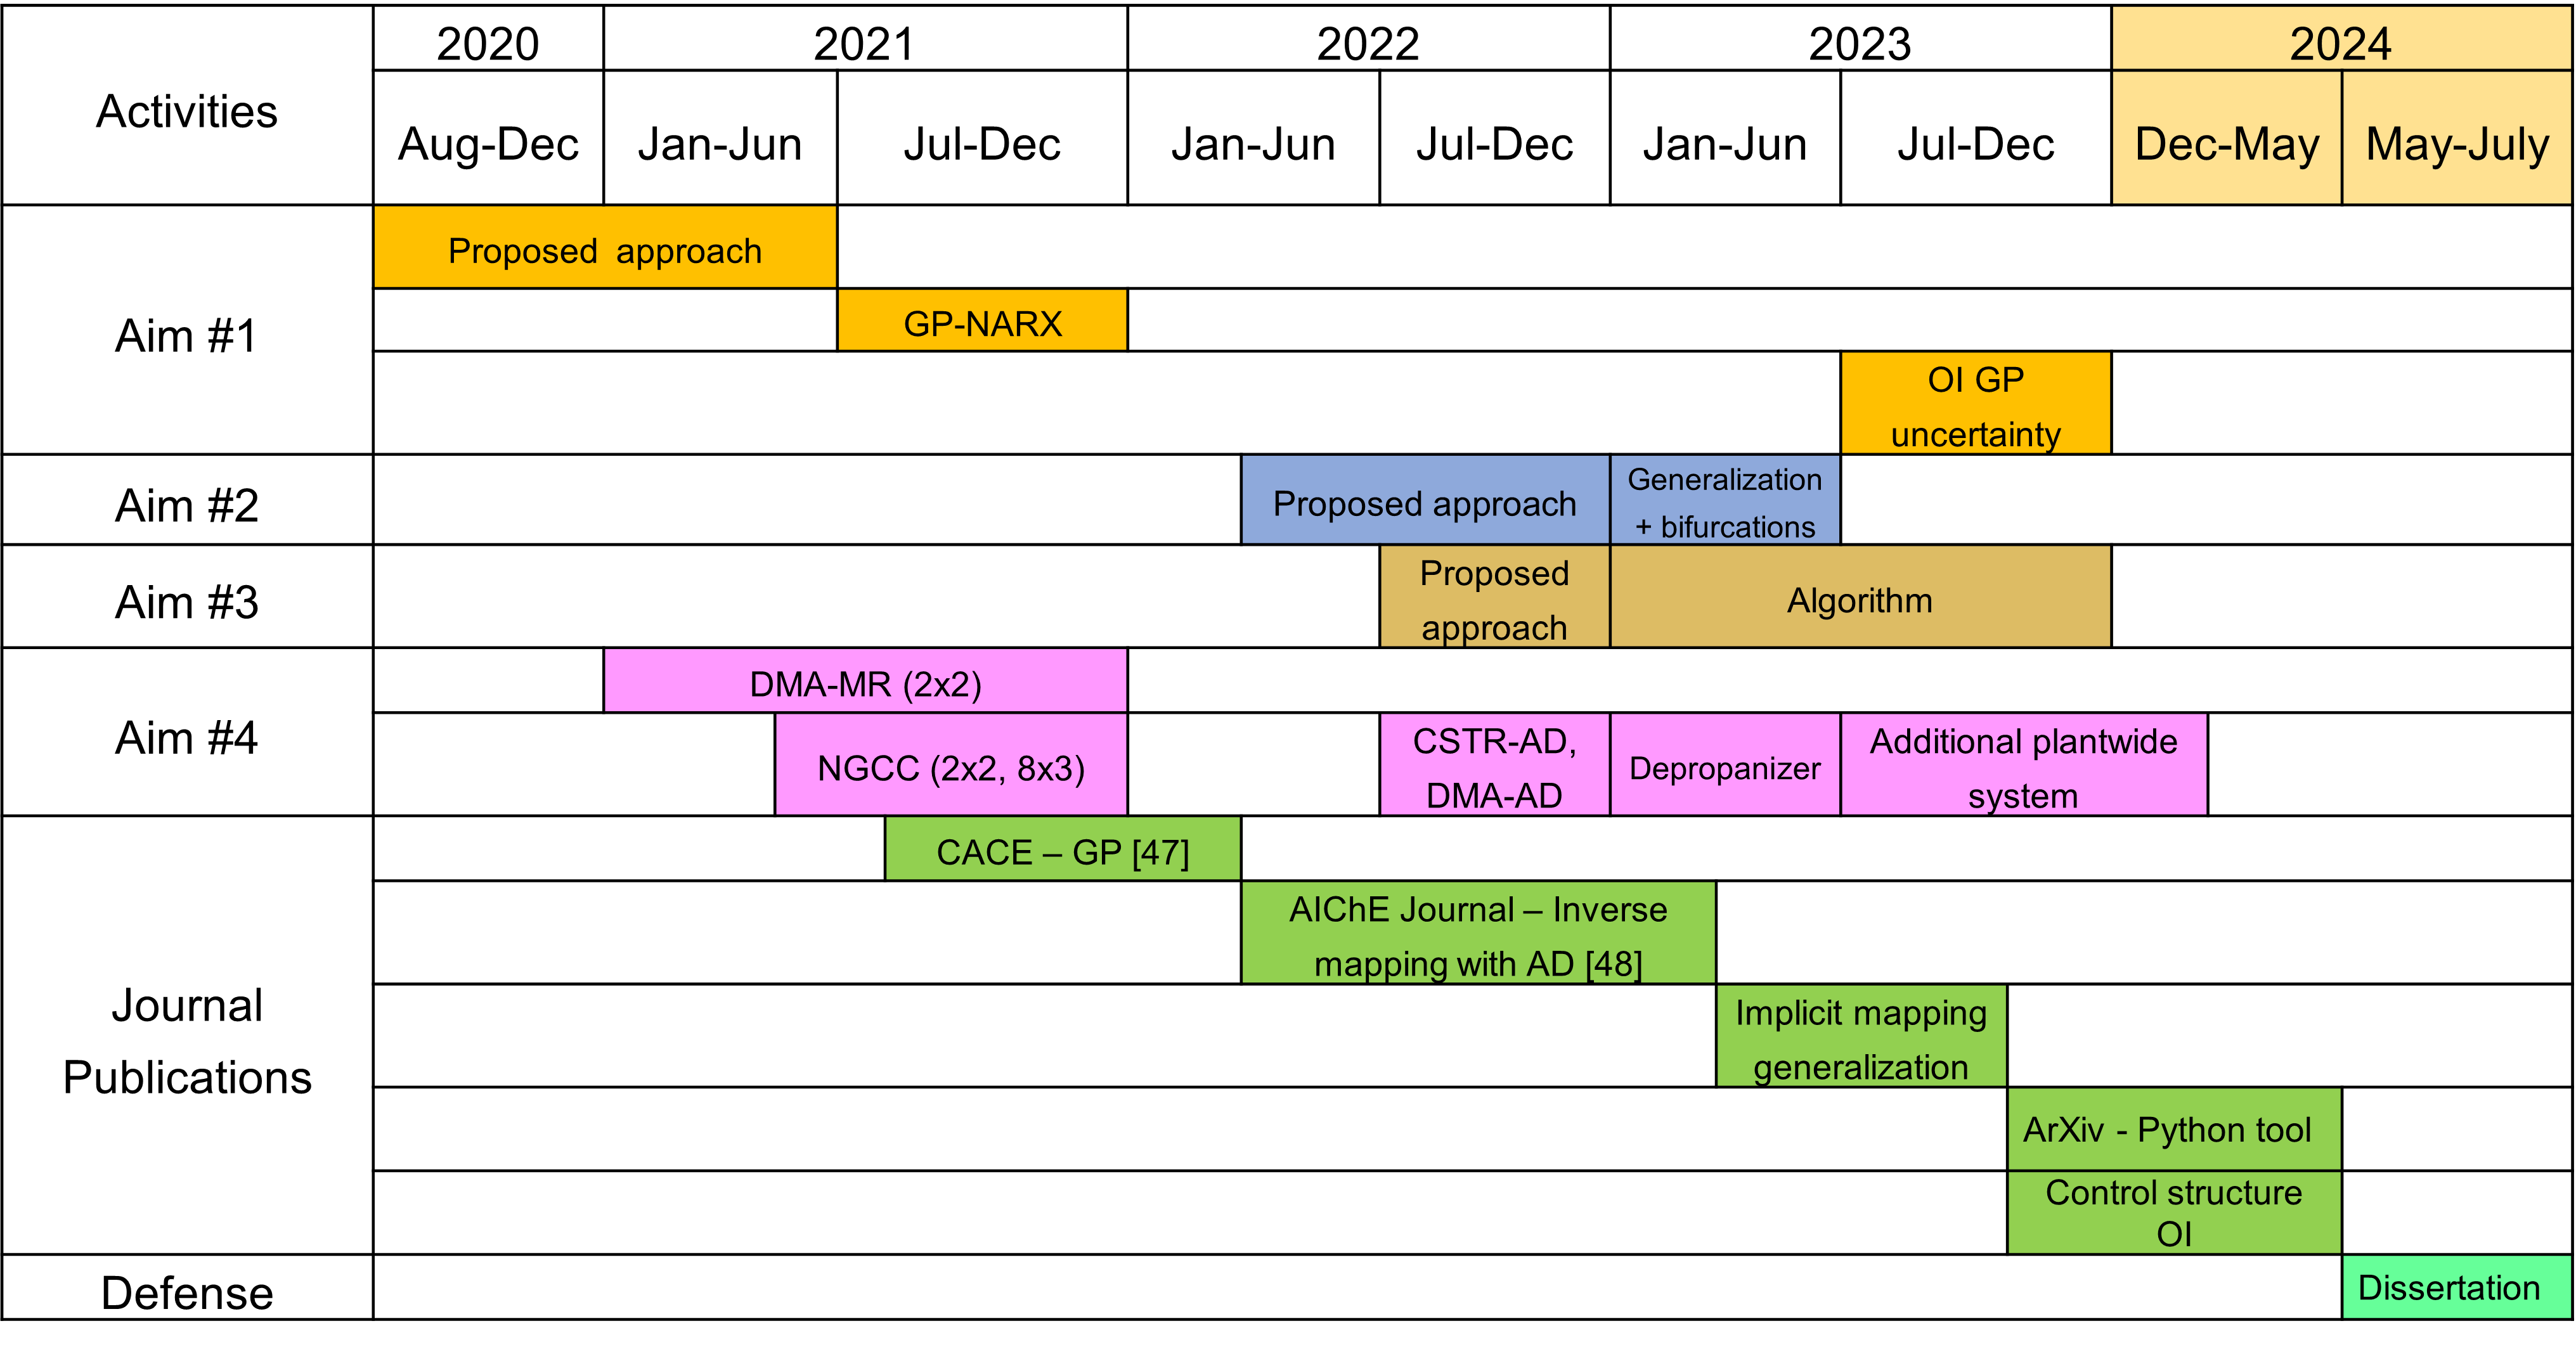
\includegraphics[width=0.95\textwidth]{research_plan.png}}
    \caption{Research Timeline.}
    \label{timeline:timeline_table}
\end{figure}


\section*{References}
\addcontentsline{toc}{chapter}{References}
\printbibliography[heading=none]

\end{document}